\chapter{Results}
\section{Users}
  In total, 15 people participated in the user study.
  They were recruited from MIT students,
  via dorm and living group mailing lists.

  All of the 15 people participated in the opening and closing interviews.
  However, only 8 of them participated in the Android portion of the study.
  The reasons for this will be discussed in the Section \ref{sec:Android}.

  The participants were compensated for their degree of participation,
  and the compensation structure is outlined in Table \ref{table:compensation}.
  in Appendix A.

\section{Opening Questionnaire Results}
  The results from the opening questionnaire help to characterize the group's
  general thoughts on the subject of stress and support.
  
  Part of the survey included questions, scored on a Likert Scale,
  addressing to what degree they reach out to friends or family when troubled,
  and to what degree they feel supported by friends and family.
  The results are shown in Figure \ref{fig:likert}.

    \begin{figure}
    \centering
    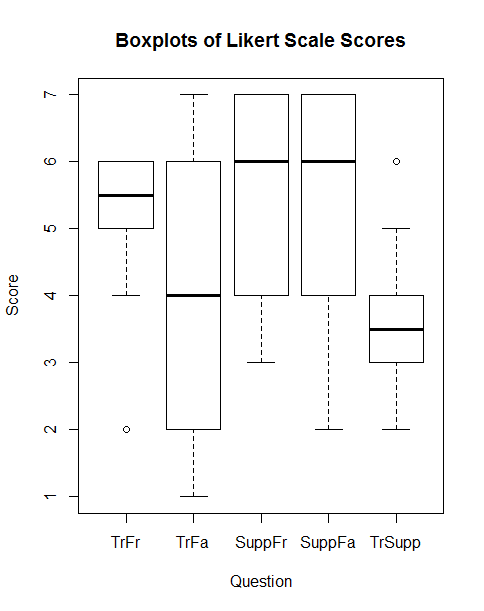
\includegraphics[width=0.6\textwidth]{likert.png}
    \caption[Likert Scale Box Plots]{
      Results of Likert scale styled questions on the opening questionnaire.
      TrFa and TrFa asked whether participants want to talk to
      Friends or Family when Troubled.
      SuppFa and SuppFa asked whether participants felt supported by
      Friends or Family.
      TrSupp asked if they reached out, in general, when troubled.
    }
    \label{fig:likert}
    \end{figure}

  Also in the opening questionnaire, we administered a Perceived Stress Scale.
  The results, shown in a histogram in Figure \ref{fig:perceived_stress},
  show that in general, the users in this study had relatively low
  self-reported stress.

    \begin{figure}
    \centering
    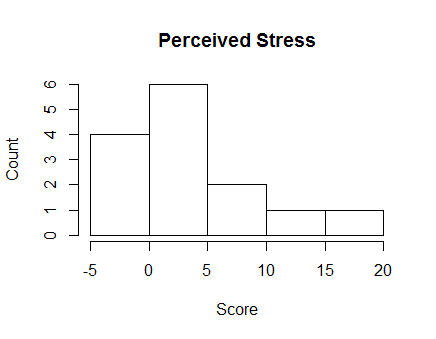
\includegraphics[width=0.6\textwidth]{perceived_stress.png}
    \caption[Perceived Stress]{
      Distribution of Perceived Stress scores amongst the 15 participants.
    }
    \label{fig:perceived_stress}
    \end{figure}

\section{Opening Interview: Script Based Results}
  The opening interview, as mentioned in Section \ref{sec:opening_int},
  followed a script, so I'll briefly outline some of the
  prominent results from the 5 sections.

  \subsection{Support-Interest}
  Because the participants' situations were so different,
  the degree to which they wanted or needed social support were very different as well.
  I assessed their general degree of need and interest in reaching out,
  what I call support-interest, during the interview.
  I define support-interest as the trait of consistently having a desire
  and making efforts to
  connect on an emotional and empathetic level with loved ones.
  Based on the nature of their support network
  and how they choose to interact with the members in it,
  it is relatively straightforward to characterize the interviewee's
  current level of support-interest.
  From the interviewees descriptions, support-interest isn't an inherent trait,
  and is instead also dependent upon the current situation of the interviewee.

  Interviewees on the low support-interest end
  have a preference for keeping their concerns to themselves.
  Two interviewees seemed especially independent,
  expressing a desire for and general pattern of dealing with things alone,
  without much external input.
  They were by no means not social.
  Both reported having plenty of friends that they interacted with regularly,
  but they chose to keep them at a greater distance when it came to things
  they were particularly sensitive about.
  When asked
  about how they discuss serious subjects with those closest to them,
  they tend to express a lack of interest.
  A quote from one of them
  helps to express the sentiment:
  \begin{itemize}
  \item
  \textit{
  ``[These thoughts are] my personal complications.
  I usually don't share that much with people because
  I'm not comfortable with them knowing me too well.
  I prefer to keep a personal boundary."
  }
  - Participant 1847, on her thoughts about keeping her privacy,
  \end{itemize}

  On the high support-interest end, there was a lot of variability.
  High support-interest people included my married interviewees, who notably,
  married within the last 5 years or so,
  and expressed being very open with their spouses, sharing everything.
  They also included a participant very active in her church community,
  and other individuals close with their parents or significant others.
  These participants expressed spending a lot of time invested in
  sharing feelings and struggles.
  Quotes associated with them included:
  \begin{itemize}
  \item \textit{
  ``She was the first person that I felt like I could talk freely with.
  We can talk about anything and everything.
  She asks questions that really pin at trying to figure out
  where emotions are coming from, what's really bothering me at a certain time.
  Just the fact that she lets me talk freely and with understanding
  makes me more comfortable."
  }
  - Participant 8594, about her mentor figure.
  \item \textit{
  ``I talk most to my mom... I try to tell my mom everything.
  She's not pushy, but she won't let me not tell her things.
  She'll ask `And then what did the the doctor say? And then?
  What's this medicine? I need to look it up!'
  [So] then I tell her everything, because she worries."
  }
  - Participant 1496, about her mother.
  \item  \textit{
  ``We're on GChat a lot.
  We chat throughout the day.
  I know how she's feeling with about a 15 minute resolution."
  }
  - Participant 3792, about his girlfriend.
  \item \textit{
  ``I have a really honest relationship with [boyfriend name].
  He'll be the first one to check in after a medical appointment,
  so is most aware...
  Rather than him trying to make sense of it,
  it makes more sense for him to just be supportive and be there.
  ... If I say anything negative, he'll jump on it.
  If I'm feeling down on myself,
  just him kinda being, `Hey, you're doing the best you can.'
  ... Sometimes I'm in the place to hear it."
  }
  - Participant 4416, about her boyfriend.
  \item \textit{
  ``I have a group of two women.. we call ourselves accountability partners.
  We meet up, like, every week.
  The idea of keeping each other accountable is
  [about] committing to listen to one another, encourage one another,
  and challenge one another to live a life of faith."
  }
  - Participant 5397, about her certain members of her church community.
  \end{itemize}

  \subsection{Choosing People and Choosing Topics}
  On discussing the support network of the interviewees,
  they tended to have a certain group of people that they turned to for
  general day-to-day support.
  These people could be family, or family-like people, as well as friends,
  but most times, participants had a strong preference towards one or the other.

  In most cases, the interviewee chose to discuss serious subjects ---
  about things that were really on their minds ---
  with only friends or only family,
  and chose to discuss only mundane, less serious topics with the other.
  For example, Participant 1010, talking about her parents,
  expressed a common sentiment.
  \textit{
  ``We only talk about mundane things...
  things not directly related to life."
  }

  \subsection{Serious Situation}
  Although the call for participant recruitment called for participants
  dealing with some serious situation in their lives,
  whether mourning or illness or other unusual difficulty of transition,
  the severity of the participants' situations varied.

  On the lighter end of the spectrum included six participants who were
  dealing with regular academic and career pressures.
  On the heavier end,
  three participants were dealing with very serious chronic illnesses,
  another was bereaved,
  and others were battling other forms of daunting transitions and trials.

  \subsection{Meeting Needs}
  Luckily, all of my participants who wanted support had people
  who could provide it.
  However, as anticipated by other research \cite{skeels10},
  when the needs grew, it became harder for some of my participants to get
  what they needed.

  Participant 9541 expressed a general sentiment about discussing tough topics:
  \textit{
  ``Feeling like you need it and actually reaching out are two different things.
  It's a lot harder to say `I'm struggling with whatever's going on.'"
  } and Participant 5397 described a high learning curve
  \textit{
  ``Two years ago.
  Actually, even a year ago, I was not very good about reaching out to people.
  It takes a lot of energy to reach out to people and explain what's going on.
  [We thought]
  `If these people are really my friends, they should be reaching out to me,'
  but actually, if they don't know, they don't know.
  Nowadays, there's a group of people we'll email or call.
  Maybe we should be asking a few people, specifically, to be on-call."
  }

  \subsection{Technology}
  On technology,
  my participants tended to be technically savvy.
  This is likely due to the age range of the participants,
  the youngest of which was 18, and the oldest 30.
  Consistent with previous research,
  they used a complex range of technologies to connect
  with friends and family near and at distance,
  for a range of complicated reasons.

  More convenient forms of communication,
  such as text or other forms of instance message,
  were used frequently for casual things such as keeping in touch,
  and other modes of communication, such as video, phone, or in person meetings,
  were used for more serious topics.
  The exception to this was email,
  which despite being digital and text based, 
  afforded a level of thoughtfulness that participants
  felt were especially valuable in a different way.
  One participant found emails the best medium for reconnecting
  with distant friends on the nature and current condition of her
  chronic illness,
  and another participant who had depressive episodes found that
  email communications fell better into her comfort zone during the dark times.

\section{Opening Interview: Other Trends}
  The trends addressed by the script of the opening interview touched on
  some important topics, but the most interesting results
  were other patterns and phenomena
  that were not anticipated by the script.

  \subsection{Direction of Awareness}
  In many cases, there was a clear directionality to the type of awareness
  information shared.
  One recurrent example was with parents,
  when the daughter or son tends to report a lot to the parent,
  and the parent reports relatively little in return.
  Other relationships, such as between siblings or friends,
  can also be very directional,
  with one party in the habit of disclosing more to the other.
  for example, Participant 1010 explained her relationships:
  \textit{
  ``With some of my friends, I like to know what they're doing.
  I kinda mother them.
  I like to make sure they're doing okay."
  }

  \subsection{Extreme Information Withholding}
  Another phenomenon that became apparent with interviews is that
  many, even normally trusting, close relationships,
  can incorporate extreme instances of information withholding.
  One relatively whimsical example was brought up
  when the topic of awareness and updates from family was brought up.
  \textit{
    ``
    They don't tell me anything. No.
    They feel like I should focus on me.
    Even when my dog passed away, they didn't tell me for an entire month.
    They didn't want me to be upset.
    I just noticed the dog wasn't there, and they never straight up told me."
  } - Participant 2928

  It's important to note that the story is one instance of a general
  trend of not sharing bad news.
  This can be as simple as preferring to look on the bright side:
  \textit{
  ``I try to look on the bright side.
  For example, my Facebook page used to be full of sad things.
  I decided not to do that anymore."
  } - Participant 3792
  or \textit{
  ``[My struggles are] not really fun to talk about.
  Most people already have enough on their plate"
  }
  - Participant 9451
  
  This can also be taken to the extreme.
  One specific example from my participants involved
  completely not telling family members about a serious issue,
  while maintaining communications otherwise.

  \subsection{Changes in Support Structure}
  Lastly, closely related to the extreme information withholding,
  there are many situations in our lives that result in
  drastic changes in the nature of our support structure.
  As mentioned in Section \ref{sec:intro},
  death can be the most tragic cause of such a change.
  When the person who passed away had a pivotal role in the support
  structure of another, it can be even harder to cope with
  the difficult period of mourning.
  Though this was true for a participant who was bereaved,
  the drastic changes that other interviewees described usually involved
  a falling out of some sort.
  These falling outs could be between family members,
  significant others, or even friends,
  and completely overturn an existing network.

\section{Android}
  After the Opening Interview, participants were instructed to invite
  at least 2 people to join their group.
  Once there were 3 people in a group,
  they were given the InMind application,
  and they could begin.

  \section{Weekly Feedback}
  Most of the weely feedback consisted of feature requests.
  Some participants wanted to be able to change the sharing status
  of a topic after it was started.
  Others wanted to be able to post pictures onto a topic.

  \section{Data and Questions to Answer}
    Since the data set only includes 8 groups,
    it is not particularly meaningful to derive any statistical conclusions
    from them.
    However, a data set of 8 groups, 36 users, 70 topics, and 1111 messages
    is still useful for observing some likely trends.
    The questions that I will discuss in this section are the following:
    \begin{enumerate}
      \item When are topics made?
      \item How many topics are made in each week?
      \item How many messages are sent each week?
      \item Who receives topics?
      \item How long does a topic live?
      \item How much time is spent on the app?
      \item How much of that is with individual plants/writing notes?
      \item What time of day is the app accessed?
      \item For browsing vs status updating?
    \end{enumerate}

    Topics are created generally in the mornings and evenings,
    presumably before the day starts and after the day ends,
    and not when things are happening.
    The distribution of hours of creation is shown in
    Figure \ref{fig:topic_hours},
    which shows a bimodal distribution centered on waking and sleeping hours.

    \begin{figure}
    \centering
    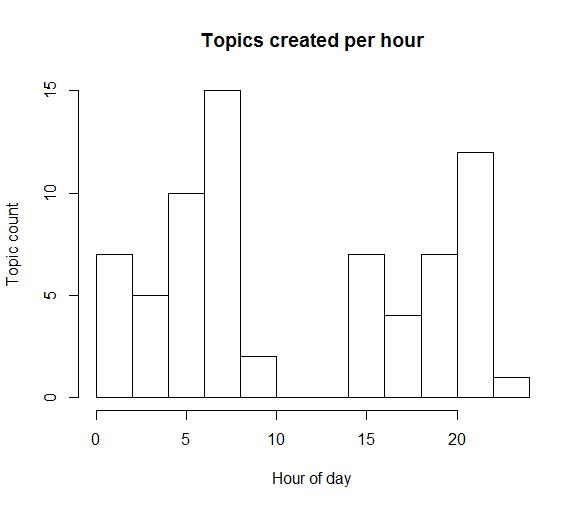
\includegraphics[width=0.6\textwidth]{topics_per_hour.jpg}
    \caption[Topics Created by Hour of Day]{
      Topics were created at varying hours of the day.
      The 70 topics shown in this bar chart appear to show
      topics being created in the morning and evenings,
      and occasionally in late evening/early morning,
      but fewer in the middle of the day, between 10:00 A.M. and 3:00 P.M.
    }
    \label{fig:topic_hours}
    \end{figure}

    After the opening interviews, we looked at the types of stressors the
    interviewees faced, and postulated likely types of topics.
    Before we began the three week study,
    we hypothesized that there were generally 2 types of topics,
    short lived and long lived ones.
    Short lived topics we imagined would last a few days to a week,
    and would include things like class projects,
    work deadlines, short conflicts with friends, and other temporary frustrations.
    Long lived topics we imagined would last much longer,
    and would include the more serious topics, likely the major stressor,
    and since these stressors are expected to last several months to indefinitely,
    should remain active for the duration of the 3 week study.
    This ended up remarkably accurate,
    but we had not anticipated that many topics would be created,
    and never become active.
    These "zero-day" topics were created,
    but were neither updated nor discussed after the day they were created.

    In Figure \ref{fig:topic_age}, charts show two different measures of 
    topic duration, filtered and not filtered to remove the zero-day topics.

    \begin{figure}
    \centering
    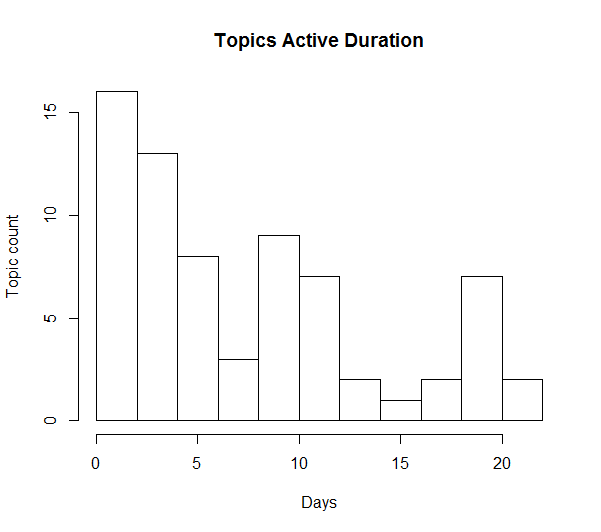
\includegraphics[width=0.6\textwidth]{topic_days_active.png}
    \caption[Duration of Topics] {
      Topics were active for varying periods.
    }
    \label{fig:topic_age}
    \end{figure}


\begin{table}[h]
\centering
\caption{Compensation Chart}
\label{table:compensation}
\begin{tabular}{ l l }
Task & Compensation \\
\hline
Opening Interview & \$10 \\[5pt]
Android Week 1 & \$5 \\[5pt]
Android Week 2 & \$5 \\[5pt]
Android Week 3 & \$5 \\[5pt]
Android Week All & \$25 \\[5pt]
Closing Interview & \$10 \\[5pt]
\hline
Total & \$60
\end{tabular}
\end{table}


    


  \section{Attrition}
  \label{sec:Android}
  Of the 15 participants, 2 could not continue the Android portion
  of the study due to timing constraints.
  5 more did not get two people in their group,
  so after two weeks,
  we decided to call them in for a closing interview.
  *TBD INSERT PSEUDO CLOSING INTERVIEW MATERIAL*

